%%%%%%%%%%%%%%%%%%%%%%%%%%%%%%%%%%%%%%%%%%%%%%%%%%%%%%%%%%%%%
% \subsection{Глоссарий}
% \begin{frame}[c]
% 	\frametitle{Введениe}
% 	\begin{spacing}{1}
% 		\begin{enumerate}
% 			\item \textbf{Нейрон} – клетка, главное рассматриваемое свойство которой -- способность к генерации импульса возбуждения
% 			\item \textbf{Подпороговые колебания} – колебания квазигармонического типа, спонтанно возникающие в нейроне
% 			\item \textbf{Спайк} – единичный импульс, генерируемый нейроном как отклик на внешнее воздействие выше порога возбуждения
% 			\item \textbf{Спайк-берст} – режим колебаний, при котором на одном высоком периоде генерируется больше одного спайка  
% 		\end{enumerate}
% 		\vspace{1em}
% 		Способность нейрона к подпороговым колебаниям и генерации импульсов отражена в рассматриваемой модели.
% 	\end{spacing}
% \end{frame}
%%%%%%%%%%%%%%%%%%%%%%%%%%%%%%%%%%%%%%%%%%%%%%%%%%%%%%%%%%%%%
% \section{Теоретическая часть}
% \subsection{Подпороговые колебания в нейронах}
% \begin{frame}[c]
% 	\frametitle{Подпороговые колебания в нейронах}
% 	\begin{columns}
% 		\begin{column}{0.49\textwidth}
% 			\begin{figure}[h]
% 				\centering
% 				\includegraphics[]{img/img_1a}
% 				\caption[]{Различные виды колебаний в нейронах ствола головного мозга \cite{linas}}
% 			\end{figure}
% 		\end{column}
% 		\begin{column}{0.49\textwidth}
% 			\begin{figure}[h]
% 				\centering

% 				\includegraphics[]{img/img_1d}	
% 				\caption[]{Зависимость динамики колебаний в нейронах коры головного мозга от тока стимуляции\cite{linas}}
% 			\end{figure}
% 		\end{column}
% 	\end{columns}
% \end{frame}
% %%%%%%%%%%%%%%%%%%%%%%%%%%%%%%%%%%%%%%%%%%%%%%%%%%%%%%%%%%%%%
% \subsection{Генератор Ван-дер-Поля: фазовый портрет}
% \begin{frame}[t]
% 	\frametitle{Генератор Ван-дер-Поля: фазовый портрет}
% 	\vspace{-1.2em}
% 	% \vspace{1em}
		
% 	\begin{columns}
% 		\begin{column}{0.49\textwidth}
% 			\begin{figure}[h]
% 				\centering
% 				\includegraphics[scale=0.99]{img/img_2a}
% 				\caption{$\gamma<0$:\\ устойчивый фокус}
% 			\end{figure}
% 		\end{column}
% 		\begin{column}{0.49\textwidth}
% 			\begin{figure}[h]
% 				\centering
% 				\includegraphics[scale=0.99]{img/img_2b}
% 				\caption{$\gamma>0$:\\ предельный цикл}
% 			\end{figure}
% 		\end{column}
% 	\end{columns}	
% 	\vspace{0.5em}
% 	\begin{columns}[c]
% 		% \begin{column}{0.49\textwidth}
% 		% \centering
% 		% В данной системе реализуются подпороговые колебания:
% 		% % При $\gamma=0$ происходит бифуркация Андронова-Хопфа и рождается предельный цикл
% 		% \end{column}
% 		\begin{column}{0.99\textwidth}
% 	\begin{equation*}
% 		\left\{
% 		\begin{aligned}
% 			\diff{y}{t} & =\mu(\gamma-x^2)y-\omega^2x\\%; \qquad
% 			\diff{x}{t}  &=y, \quad \mu \ll 1
% 		\end{aligned}
% 		\right.
% 	\end{equation*}		
% 		\end{column}
% 	\end{columns}
% \end{frame}
% %%%%%%%%%%%%%%%%%%%%%%%%%%%%%%%%%%%%%%%%%%%%%%%%%%%%%%%%%%%%%
% \subsection{Модель ФитцХью-Нагумо: фазовый портрет}
% \begin{frame}[t]
% 	\frametitle{Модель ФитцХью-Нагумо: фазовый портрет}
% 	% Способность к генерации спайков реализуется с помощью модели ФХН. Это простейшая система, обладающая порогом возбуждения:
% 	% \vspace{1em}
% 	\begin{columns}[c]	
% 		\begin{column}{0.59\textwidth}
% 			\vspace{-2em}
% 			\begin{figure}[h]
% 				\centering
% 				\hspace{1em}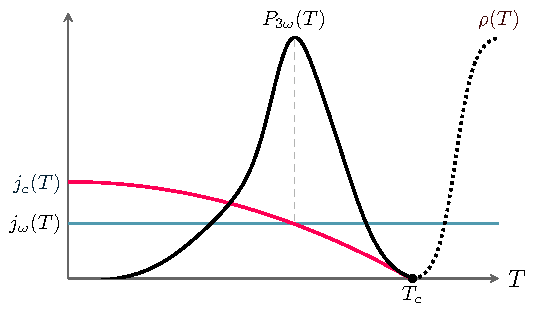
\includegraphics[]{img/img_3a}
% 				% \caption{3-уровневая среда}
% 			\end{figure}
% 			\vspace{-2em}
% 			\begin{figure}[h]
% 				\centering
% 				\hspace{1em}\includegraphics[]{img/img_3b}
% 				% \caption{3-уровневая среда}
% 			\end{figure}
% 		\end{column}
% 		\begin{column}{0.39\textwidth}
% 			$
% 				\left\{
% 				\begin{aligned}
% 					\diff{u}{t} & =f(u)-v           \\
% 					\diff{v}{t} & =\varepsilon(u-I)
% 				\end{aligned}
% 				\right.
% 			$\\
% 			\vspace{1em}
% 			$I$ -- параметр порога возбуждения\\
% 			\vspace{1em}
% 			$f(u)$ -- кубическая функция\\
% 			\vspace{1em}
% 			$\varepsilon \ll 1$ -- малый параметр
% 		\end{column}
% 	\end{columns}
% \end{frame}
% %%%%%%%%%%%%%%%%%%%%%%%%%%%%%%%%%%%%%%%%%%%%%%%%%%%%%%%%%%%%%
% \subsection{Компьютерная модель Некоркина}
% \begin{frame}%[bg]
% 	\frametitle{Математическая модель нейрона}

% 		% \vspace{-1em}
	
% 	\begin{columns}[b]
% 		\begin{column}{0.60\textwidth}
% 			% \vspace{-3em}
% 			\begin{equation*}
% 				\left\{
% 				\begin{aligned}
% 					\varepsilon_1\diff{u}{t} & =f(u)-v-d\cdot x\\
% 					\diff{v}{t} & =\varepsilon_2(u-I)\\
% 					\diff{x}{t} & =y\\
% 					\diff{y}{t} & =\mu(\Gamma(u,I)-x^2)y-\omega^2\cdot x
% 				\end{aligned}
% 				\right.
% 			\end{equation*}
% 		\end{column}
% 		\begin{column}{0.40\textwidth}
% 			$f(u)=u(1-u)(u-a)$\\
% 			\vspace{0.7em}
% 			$\Gamma(u,I)=\gamma(1-\alpha I +\beta u)$\\
% 			\vspace{0.7em}
% 			\begin{columns}[t]
% 			\begin{column}{0.49\textwidth}
% 				$a=0.1$\\
% 				$\varepsilon_1=0.001$\\
% 				$\varepsilon_2=1.5$\\
% 				$\gamma=0.21$\\
% 				$\omega=1$\\
% 			\end{column}
% 			\begin{column}{0.49\textwidth}
% 				$\alpha=5$\\
% 				$\beta=10$\\
% 				$I=-0.09$\\
% 				$d=0.85$\\
% 			\end{column}			
% 			\end{columns}
% 		\end{column}
% 	\end{columns}
% 	\begin{figure}[h]
% 		% \hspace{-2em}
% 		\includegraphics[scale=1]{img/limit}
% 		% \caption{}
% 	\end{figure}
% \end{frame}
% %%%%%%%%%%%%%%%%%%%%%%%%%%%%%%%%%%%%%%%%%%%%%%%%%%%%%%%%%%%%%
% \subsection{Характерные режимы модели}
% \begin{frame}%[bg]
% 	\frametitle{Характерные режимы модели}
% 		% \vspace{-2em}
% 	\begin{figure}[h]
% 		\hspace{0em}
% 		\includegraphics[scale=1]{img/img_4}
% 		% \caption{}
% 	\end{figure}
	
% 	% \begin{columns}[t]
% 	% 	\begin{column}{0.60\textwidth}
% 	% 		\vspace{-3em}
% 	% 		\begin{equation*}
% 	% 			\left\{
% 	% 			\begin{aligned}
% 	% 				\varepsilon_1\diff{u}{t} & =f(u)-v-d\cdot x\\
% 	% 				\diff{v}{t} & =\varepsilon_2(u-I)\\
% 	% 				\diff{x}{t} & =y\\
% 	% 				\diff{y}{t} & =\mu(\Gamma(u,I)-x^2)y-\Omega^2(u,I)\cdot x
% 	% 			\end{aligned}
% 	% 			\right.
% 	% 		\end{equation*}
% 	% 	\end{column}
% 	% 	\begin{column}{0.2\textwidth}
% 	% 		$a=0.1$\\
% 	% 		$\varepsilon_1=0.001$\\
% 	% 		$\varepsilon_2=1.5$\\
% 	% 		$\gamma=0.21$\\
% 	% 		$\omega=1$\\
% 	% 	\end{column}
% 	% 	\begin{column}{0.19\textwidth}
% 	% 		$\alpha=5$\\
% 	% 		$\beta=10$\\
% 	% 		$I=-0.09$\\
% 	% 		$d=0.85$\\
% 	% 	\end{column}		
% 	% \end{columns}
% \end{frame}
% %%%%%%%%%%%%%%%%%%%%%%%%%%%%%%%%%%%%%%%%%%%%%%%%%%%%%%%%%%%%%
% \subsection{Схема экспериментальной установки}
% \begin{frame}[t]%[bg]
% 	\frametitle{Схема экспериментальной установки}
% 	\vspace{-1em}
% 	\begin{figure}[h]
% 		% \hspace{-2em}
% 		\includegraphics[width=0.86\linewidth]{img/img_6}
% 		% \caption{}
% 	\end{figure}
% 	\vspace{-0.5em}
% 	\begin{columns}
% 		\begin{column}{0.49\textwidth}%\centering
% 			\sq{black!90} -- генератор Ван-дер-Поля\\
% 			\sq{red} -- эмиттерный повторитель
% 		\end{column}
% 		\begin{column}{0.49\textwidth}%\centering
% 			\sq{blue} -- эмиттерный повторитель\\
% 			\sq{lightgreen} -- блокинг-генератор
% 		\end{column}
% 	\end{columns}		
% \end{frame}
% %%%%%%%%%%%%%%%%%%%%%%%%%%%%%%%%%%%%%%%%%%%%%%%%%%%%%%%%%%%%%
% \section{Результаты эксперимента}
% \subsection{Подпороговые колебания}
% \begin{frame}%[bg]
% 	\frametitle{Подпороговые колебания}
% 	\begin{figure}[h]
% 		\hspace{-2em}
% 		\includegraphics[]{img/osci}
% 		% \caption{}
% 	\end{figure}
% \end{frame}
% %%%%%%%%%%%%%%%%%%%%%%%%%%%%%%%%%%%%%%%%%%%%%%%%%%%%%%%%%%%%%
% \subsection{Один спайк на несколько периодов}
% \begin{frame}%[bg]
% 	\frametitle{Один спайк на несколько периодов}
% 	\begin{figure}[h]
% 		\hspace{-2em}
% 		\includegraphics[]{img/spike}
% 		% \caption{}
% 	\end{figure}
% \end{frame}
% %%%%%%%%%%%%%%%%%%%%%%%%%%%%%%%%%%%%%%%%%%%%%%%%%%%%%%%%%%%%%
% \subsection{Один спайк на период}
% \begin{frame}%[bg]
% 	\frametitle{Один спайк на период}
% 	\begin{figure}[h]
% 		\hspace{-2em}
% 		\includegraphics[]{img/onespike}
% 		% \caption{}
% 	\end{figure}
% \end{frame}
% %%%%%%%%%%%%%%%%%%%%%%%%%%%%%%%%%%%%%%%%%%%%%%%%%%%%%%%%%%%%%
% \subsection{Два спайка на периоде}
% \begin{frame}%[bg]
% 	\frametitle{Два спайка на периоде}
% 	\begin{figure}[h]
% 		\hspace{-2em}
% 		\includegraphics[]{img/twospike}
% 		% \caption{}
% 	\end{figure}
% \end{frame}
% %%%%%%%%%%%%%%%%%%%%%%%%%%%%%%%%%%%%%%%%%%%%%%%%%%%%%%%%%%%%%
% \subsection{Спайк-берст}
% \begin{frame}%[bg]
% 	\frametitle{Спайк-берст}
% 	\begin{figure}[h]
% 		% \hspace{-1.3em}
% 		% \centering
% 		\hspace{-2em}
% 		\includegraphics[]{img/berst}
% 		% \vspace{-1.5em}
% 		% \caption{Эксперимент}
% 	\end{figure}
% 	% \begin{figure}[h]
% 	% % \vspace{-1em}
% 	% 	% \hspace{-2em}
% 	% 	\centering
% 	% 	\includegraphics[]{img/berst_matlab}
% 	% 	% \vspace{-1.5em}
% 	% 	\caption{Компьютерная модель}
% 	% \end{figure}	
% \end{frame}
% %%%%%%%%%%%%%%%%%%%%%%%%%%%%%%%%%%%%%%%%%%%%%%%%%%%%%%%%%%%%%
% \subsection{Влияние потенциала запирания $b_0$}
% \begin{frame}%[bg]
% 	\frametitle{Влияние потенциала запирания $b_0$}
% 	\begin{figure}[h]
% 		% \hspace{2em}
% 		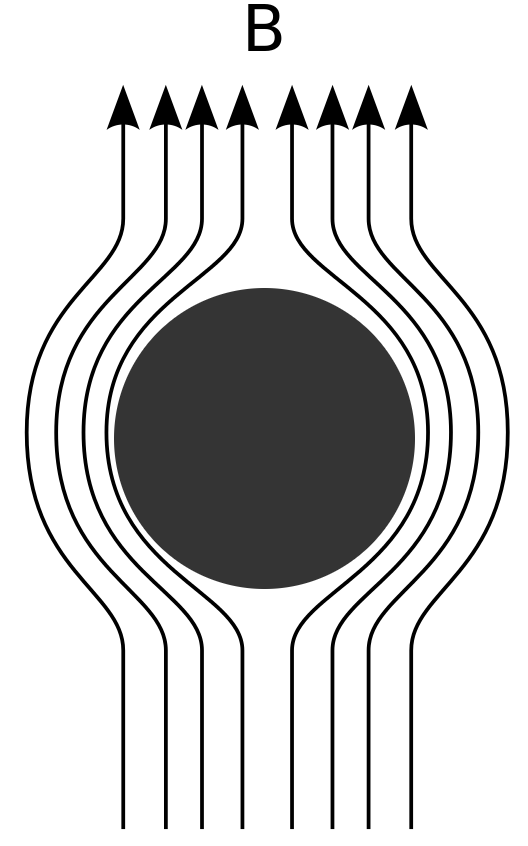
\includegraphics[]{img/b0}
% 		\caption{Зависимость частоты спайков от величины \\потенциала запирания $b_0$ }
% 	\end{figure}
% \end{frame}
% %%%%%%%%%%%%%%%%%%%%%%%%%%%%%%%%%%%%%%%%%%%%%%%%%%%%%%%%%%%%%